\noindent 
In this unit you will learn how to...
\begin{enumerate}
\item Define, draw, and explain what a vector is in 2 and 3 dimensions.
\item Add, subtract, multiply (scalar, dot product, cross product) vectors. Be able to illustrate each operation geometrically.
\item Use vector products to find angles, length, area, projections, and work.
\item Use vectors to give equations of lines and planes, and be able to draw lines and planes in 3D.
\end{enumerate}

\clearpage

\normalsize
\section{Vectors and Lines}
\textbf{Topical Objectives:}
\begin{itemize}
\item understand vectors as quantities having length and direction, independent of position
\item express curves with parametric (vector) equations
\end{itemize}

Learning to work with vectors will be key tool we need for our work in high dimensions.  Let's start with some problems related to finding distance in 3D, drawing in 3D, and then we'll be ready to work with vectors.
`

\begin{problem}
\instructor{\\Pre-Class Recommended\\}
To find the distance between two points $(x_1,y_1)$ and $(x_2,y_2)$ in the plane, we create a triangle connecting the two points.  The base of the triangle has length $\Delta x=(x_2-x_1)$ and the vertical side has length $\Delta y=(y_2-y_1)$. The Pythagorean theorem gives us the distance between the two points as $\sqrt{\Delta x^2+\Delta y^2}=\sqrt{(x_2-x_1)^2+(y_2-y_1)^2}$.\\

\begin{enumerate}
\item Draw a 3-D axis then plot the points $(1,5)$ and $(2,3)$
\item Sketch the triangle that connects these two points and the origin -- $(0,0)$
\item Find $\Delta x$ and $\Delta y$
\item Now extend your picture into 3 and use it to show that the distance between two points $(x_1,y_1,z_1)$ and $(x_2,y_2,z_2)$ in 3-dimensions is $\sqrt{\Delta x^2+\Delta y^2+\Delta z^2}=\sqrt{(x_2-x_1)^2+(y_2-y_1)^2+(z_2-z_1)^2}$.
\item Use this formula to find the distance between the points $(1,5,2)$ and $(2,3,3)$
\end{enumerate}
\end{problem}


\begin{problem}
\instructor{\\Pre-Class Recommended\\}
\marginpar{
	\thomasee{See 12.1:41-58.} 
	\stewarts{See 12.1:11-18}
	}%end margin
Recall that a circle (or sphere in 3-D) is just a collection of points which are all equal distance away from a center point.
\begin{enumerate}
\item If the center of a circle is the point $(1,5)$ what is the equation for a circle which passes through the point $(2,3)$?
\item Find the distance between the two points $P=(2,3,-4)$ and $Q=(0,-1,1)$. 
\item Now find an equation of the sphere passing though point $Q$ whose center is at $P$. \\
Hint: Each point on the surface of a sphere is $r$ distance away from the center.
\end{enumerate}
\end{problem}


%\begin{problem}
%\marginpar{
	%\thomasee{See 12.1:1-40.} 
	%\stewarts{12.1:23-34}
	%}
%For each of the following, construct a rough sketch of the set of points in space (3D) satisfying:
%\begin{enumerate}
%\item $2\leq z\leq 5$
%\item $x=2,y=3$
%\item $x^2+y^2+z^2=25$
%\end{enumerate}
%\end{problem}

\begin{definition}
A vector is a magnitude in a certain direction.  
If $P$ and $Q$ are points, then the vector $\vec{PQ}$ is the directed line segment from $P$ to $Q$. This definition holds in 1D, 2D, 3D, and beyond.  
If $V=(v_1,v_2,v_3)$ is a point in space, then to talk about the vector $\vec v$ from the origin $O$ to $V$ we'll use any of the following notations:
$$\vec v = \vec{OV}=\left<v_1,v_2,v_3\right> 
= v_1\mathbf{i}+v_2\mathbf{j}+v_3\mathbf{k} 
= (v_1,v_2,v_3) 
= \begin{pmatrix}v_1\\ v_2\\ v_3\end{pmatrix}
.$$
The entries of the vector are called the $x$, $y$, and $z$ (or i, j, k) components of the vector. 
\end{definition}
\instructor{There are no problems actually exploring the idea of vectors NOT from the origin, i.e. between several points. This should be added or tweaked into the existing problems}
Note that $(v_1,v_2,v_3)$ could refer to either the point $V$ or the vector $\vec v$. The context of the problem we are working on will help us know if we are dealing with a point or a vector.

\begin{definition}
Let $\mathbb{R}$ represent the set real numbers. Real numbers are actually 1D vectors.\\
Let $\mathbb{R}^2$ represent the set of vectors $(x_1,x_2)$ in the plane.\\
Let $\mathbb{R}^3$ represent the set of vectors $(x_1,x_2,x_3)$ in space. There's no reason to stop at 3, so let $\mathbb{R}^n$ represent the set of vectors $(x_1,x_2,\ldots,x_n)$ in $n$ dimensions.
\end{definition}
In first semester calculus and before, most of our work dealt with problem in $\mathbb{R}$ and $\mathbb{R}^2$. Most of our work now will involve problems in $\mathbb{R}^2$ and $\mathbb{R}^3$. We've got to learn to visualize in $\mathbb{R}^3$.

\begin{definition}\label{def:vecadd}
Suppose $\vec x=\left<x_1,x_2,x_3\right>$ and $\vec y=\left<y_1,y_2,y_3\right>$ are two vectors in 3D, and $c$ is a real number. We define vector addition and scalar multiplication as follows:
\begin{itemize}
\item Vector addition: $\vec x+\vec y = (x_1+y_1,x_2+y_2,x_3+y_3)$ (add component-wise).
\item Scalar multiplication: $c\vec x = (cx_1,cx_2,cx_3)$.
\end{itemize}
\end{definition}

\begin{problem}
\marginpar{
	\thomasee{See 12.2:23-24.} 
	\stewarts{See 12.2:5-6}
	}
Consider the vectors $\vec u=\langle 1,2 \rangle$ and $\vec v=\left<3,1\right>$.  Draw $\vec u$, $\vec v$, $\vec u+\vec v$, and $\vec u-\vec v$ with their tail placed at the origin.  Then draw $\vec v$ with its tail at the head of $\vec u$. 
\end{problem}

\begin{problem}\label{prob:donkey}
\marginpar{
	\thomasee{See 11.1: 3,4.}
	}
Consider the vector $\vec v=\langle 3,-1 \rangle $.\\
\begin{enumerate}
\item Draw $\vec v$, $-\vec v$, and $3\vec v$.
\end{enumerate}
\noindent Suppose a donkey travels along the path given by $(x,y)=\vec v t = (3t,-t)$, where $t$ represents time.
\begin{enumerate}[resume]
\item At the following times, where is the donkey?
	\begin{enumerate}
		\item $t=0$ ?
		\item $t=1$ ?
		\item $t=2$ ?
	\end{enumerate}
\item Draw an axis, then sketch the path followed by the donkey. 
\item Where is the donkey at time $t=0,1,2$? Put markers with labels on your graph to show the donkey's location.
\end{enumerate}
\end{problem}

\vskip0.2in

In a previous problem (\ref{prob:donkey}) you encountered $(x,y)=(3t,-t)$.  This is an example of a function where the input is $t$ and the output is a vector $(x,y)$.  For each input $t$, you get a single vector output $(x,y)$. Such a function is called a parametrization of the donkey's path. Because the output is a vector, we call the function a vector-valued function. Often, we'll use the variable $\vec r$ to represent the radial vector $(x,y)$, or $(x,y,z)$ in 3D.  So we could rewrite the position of the donkey as $\vec r(t)=(3,-1)t$. We use $\vec r$ instead of $r$ to remind us that the output is a vector.

Let's look at another, similar problem.

\begin{problem}\label{prob:horseline}
\marginpar{
	\thomasee{See 12.2: 1.}
	}
Suppose a horse races down a path given by the vector-valued function $\vec r(t) = (1,2)t+(3,4)$. (Remember this is the same as writing $(x,y) =  (1,2)t+(3,4)$ or similarly  $(x,y)=(1t+3,2t+4)$.)
\begin{enumerate}
	\item Where is the horse at time $t=0,1,2$? 
	\item Draw an set of axis and put markers on your graph to show the horse's location.
	\item Draw the path followed by the horse.
\end{enumerate}

\end{problem}


%Day two of vectors
%\uday
%\large Topical Objectives: \normalsize \\
%\indent $\bullet$ understand vectors as quantities having length and direction, independent of position\\
%\indent $\bullet$ express curves with parametric (vector) equations\\
%\indent $\bullet$ perform addition and scalar multiplication of vectors
\instructor{Approximate end of Unit 1 : Day 1}

In the last two problems we described the donkey and horse's paths using vectors. The use of vectors actually lets us do a lot more like give a generalized direction or easily compute their speed at any point along the path. To do that we need to define two more mathematical ideas, the magnitude and unit-vector.

\begin{definition}
The magnitude, or length, or norm of a vector $\vec v = \left<v_1,v_2,v_3\right>$ is $|\vec v| = \sqrt{v_1^2+v_2^2+v_3^2}$. It is just the distance from the point $(v_1,v_2,v_3)$ to the origin.

Note that in 1D, the length of the vector $\left<-2\right>$ is simply $|-2|=\sqrt{(-2)^2}=2$, the distance to 0. Our use of the absolute value symbols is appropriate, as it generalizes the concept of absolute value (distance to zero) to all dimensions.

\end{definition}

In the special circumstance where a vector represents an object's velocity, the magnitude of the vector gives the objects \textit{speed} or non-directional velocity. 

\begin{definition} A unit vector is a vector whose length is one unit. The notation for a unit vector is generally a ``$\hat{\ }$'' or \textbf{bold face}. Equivalently, the unit vector of a vector $\vec{v}$ is: $\hat{v}=\frac{\vec{v}}{|\vec{v}|}$\\
The standard unit vectors are $\mathbf{i}=\left<1,0,0\right>$, $\mathbf{j}=\left<0,1,0\right>$, $\mathbf{k}=\left<0,0,1\right>$. 
\end{definition}

\begin{problem}[Magnitude and Unit Vector Practice]
For each of the following vectors, compute the magnitude and unit vector in the same direction.
\begin{enumerate}
	\item $-3\ii + 7 \jj$ \instructor{\# 1 Length $\sqrt{58}$}
	\item $<-4,2,4>$ \instructor{\# 2: Length - 6, Unit Vector: $<\frac{-2}{3}, \frac{1}{3}, \frac{2}{3}>$}
	\item $8\ii - \jj + 4 \kk$ \instructor{\# 3 Length 9}
\end{enumerate}
\end{problem}

\begin{problem}
\marginpar{
	\thomasee{See 12.2: 9,17,25,33 and surrounding.} 
	\stewarts{See 12.2: 23-26, 41, 42}
	}%
Consider the two points $P=(1,2,3)$ and $Q=(2,-1,0)$. 
\begin{enumerate}
	\item Write the vector $\vec {PQ}$ in component form $<a,b,c)\>$. 
	\item Find the length (magnitude) of vector $\vec {PQ}$. 
	\item Find a unit vector for $\vec{PQ}$. 
	\item Finally, find a vector of length 7 units that points in the same direction as $\vec{PQ}$. 
\end{enumerate}
\end{problem}

\begin{problem}
Let's return to problems \ref{prob:donkey} and \ref{prob:horseline}. We now have the tools to determine the donkey's and horse's speed and direction.
\begin{enumerate} 
	\item The donkey's path was given by $(x,y)=\vec v t = (3t,-t)$. Find
	\begin{enumerate}
		\item The donkey's speed
		\item A unit vector that gives the donkey's direction of travel.
	\end{enumerate}
	\item The horse's path was given by $\vec r(t) = (1,2)t + (3,4) $.
	\begin{enumerate}
		\item State the part of $\vec r(t)$ which gives the direction of travel.
		\item What is a unit vector in the same direction?
		\item what is the speed of the horse?
	\end{enumerate}
\end{enumerate}
\end{problem}


\begin{problem}
\marginpar{
	\thomasee{See 12.5: 1-12.} 
	\stewarts{Look at 12.2:34-40}
	}%
A raccoon is sitting at point $P=(0,2,3)$.  It starts to climb in the direction $\vec v=\left<1,-1,2\right>$.\\
Write a vector equation $(x,y,z)=(?,?,?)$ for the line that passes through the point $P$ and is parallel to $\vec v$. [Hint, study problem \ref{prob:horseline}, and base your work off of what you saw there. It's almost identical.] \\
Generalize your work to give an equation of the line that passes through the point $P=(x_1,y_1,z_1)$ and is parallel to the vector $\vec v=\langle v_1,v_2,v_3 \rangle$. 
\end{problem}

Make sure you ask me in class to show you how to connect the equation developed above to what you have been doing since middle school. If you can remember $y=mx+b$, then you can quickly remember the equation of a line.  If I don't show you in class, make sure you ask me (or feel free to come by early and ask before class).

%\newpage
%\noindent \Large After Class: \normalsize

\begin{problem}\label{first line between two points}%
\marginpar{
	\thomasee{See 12.5: 13-20.} 
	\stewarts{12.5: 6-15}
	}
Let $P=(3,1)$ and $Q=(-1,4)$.  
\begin{enumerate}
\item Write a vector equation $\vec r(t)=(x,y)$ for (i.e, give a parametrization of) the line that passes through $P$ and $Q$, with $\vec r(0)=P$ and $\vec r(1)=Q$.
\item Write a vector equation for the line that passes through $P$ and $Q$, with $\vec r(0)=P$ but whose speed is twice the speed of the first line.
\item Write a vector equation for the line that passes through $P$ and $Q$, with $\vec r(0)=P$ but whose speed is one unit per second.
\end{enumerate}
\end{problem}


%\uday
\section{The Dot Product}\instructor{Approximate Day 3}
\large Topical Objectives: \normalsize\\
\indent $\bullet$ perform the dot-product of two vectors\\
\indent $\bullet$ recognize when two vectors are orthogonal

\vskip0.2in

Now that we've learned how to add and subtract vectors, stretch them by scalars, and use them to find lines, it's time to introduce a way of multiplying vectors called the dot product.  We'll use the dot product to help us find find angles. First, we need to recall the law of cosines.
\begin{theorem*}[The Law of Cosines]
Consider a triangle with side lengths $a$, $b$, and $c$. Let $\theta$ be the angle between the sides of \textbf{length} $a$ and $b$. Then the law of cosines states that 
$$c^2=a^2+b^2-2ab\cos\theta.$$
If $\theta=90^\circ$, then $\cos\theta=0$ and this reduces to the Pythagorean theorem.
\end{theorem*}

\begin{problem}\instructor{Recommended as pre-class problem} 
\marginpar{
	\thomasee{See 12.3: 9-12.} 
	\stewarts{See 12.3:15-20}
	}%
Sketch in $\mathbb{R}^2$ the vectors $\left<1,2\right>$ and $\left<3,5\right>$.  Use the law of cosines to find the angle between the vectors.
\end{problem}

\begin{problem}\label{prob:dot angle practice}  \instructor{Recommended as pre-class problem}
\marginpar{
	\thomasee{See 12.3: 9-12.} 
	\stewarts{See 12.3:15-20}
	}%
Sketch in $\mathbb{R}^3$ the vectors $\left<1,2,3\right>$ and $\left<-2,1,0\right>$.  Use the law of cosines to find the angle between the vectors.
\end{problem}

\begin{definition}[The Dot Product]
If $\vec u = (u_1,u_2,u_3)$ and $\vec v= (v_1,v_2,v_3)$ are vectors in $\mathbb{R}^3$, then we define the dot product of these two vectors to be 
$$\vec u\cdot \vec v = u_1 v_1+ u_2 v_2+ u_3 v_3.$$
A similar definition holds for vectors in $\mathbb{R}^n$, where
$\vec u\cdot \vec v = u_1 v_1+ u_2 v_2+\cdots+ u_n v_n.$
You just multiply corresponding components together and then add. It is the same process used in matrix multiplication.
\end{definition}

\begin{problem}\label{prob:dot angle practice2}\instructor{Recommended as pre-class problem}
\begin{enumerate}
	\item Use the formula $\vec u\cdot \vec v=|\vec u||\vec v|\cos\theta$ to find the angle between the vectors $\left<1,2,3\right>$ and $\left<-2,1,0\right>$.
	\item Which was easier, \ref{prob:dot angle practice} or this method?  (You will derive this formula in a later problem)
\end{enumerate}
\end{problem}

\begin{definition}\label{def:orthogonal}
We say that the vectors $\vec u$ and $\vec v$ are orthogonal if $\vec u\cdot \vec v=0$. 
\end{definition}

\begin{problem}\instructor{Recommended as pre-class problem}
Find two vectors orthogonal to $(1,2)$.  Then find 4 vectors orthogonal to $(3,2,1)$.  
\end{problem}

\begin{problem}\label{dot product facts}
Mark each statement true or false. Use Definitions \ref{def:vecadd} - \ref{def:orthogonal} to explain and justify or prove your claim. You can assume that $\vec u,\vec v,\vec w\in\mathbb{R}^3$ and that $c\in\mathbb{R}$.
\begin{enumerate}
\item $\vec u\cdot \vec v=\vec v\cdot \vec u$. 
\item $\vec u\cdot (\vec v\cdot \vec w)=(\vec u\cdot\vec v)\cdot\vec w$. 
\item $c(\vec u\cdot \vec v)=(c\vec u)\cdot \vec v=\vec u\cdot (c\vec v)$. 
\item $\vec u+(\vec v\cdot \vec w)=(\vec u+\vec v)\cdot(\vec u+\vec w)$. 
\item $\vec u\cdot (\vec v+ \vec w)=(\vec u\cdot \vec v)+(\vec u\cdot\vec w)$. 
\item $\vec u\cdot \vec u= |\vec u|^2$. 
\end{enumerate}
\end{problem}

%\newpage
%\noindent \Large After Class: \normalsize

\begin{problem}\label{prob:dot prep} 
\marginpar{
	\thomasee{Page 693 has the solution if you are struggling.} 
	}
If $\vec u = (u_1,u_2,u_3)$ and $\vec v= (v_1,v_2,v_3)$ are vectors in $\mathbb{R}^3$ (which is often written $\vec u,\vec v\in\mathbb{R}^3$), then show that 
$$|\vec u-\vec v|^2 = |\vec u|^2-2\vec u\cdot \vec v +|\vec v|^2.$$
\end{problem}

\begin{problem}\label{prob:dot angle formula}  
\marginpar{
	\thomasee{See page 693.} 
	\stewarts{See pages 801-802 if you are struggling}
	}%
Let $\vec u,\vec v\in\mathbb{R}^3$. Let $\theta$ be the angle between $\vec u$ and $\vec v$. 
\begin{enumerate}
\item Use the law of cosines to explain why $|\vec u-\vec v|^2=|\vec u|^2+|\vec v|^2-2|\vec u||\vec v|\cos\theta$.
\item Use the above together with problem \ref{prob:dot prep} to derive $$\vec u\cdot \vec v=|\vec u||\vec v|\cos\theta.$$
\end{enumerate}
\end{problem}

\begin{problem} 
\marginpar{
	\thomasee{See page 694.} 
	\stewarts{See page 804}
	}%
Show that if two nonzero vectors $\vec u$ and $\vec v$ are orthogonal, then the angle between them is 90$^\circ$. Then show that if the angle between them is 90$^\circ$, then the vectors are orthogonal. I.E. expand and compute both sides of the formula $\vec u\cdot \vec v=|\vec u||\vec v|\cos\theta$ with non-zero, orthogonal vectors.
\end{problem}

The dot product provides a really easy way to find when two vectors meet at a right angle. The dot product is precisely zero when this happens.

% \begin{problem}
%   Show that the distance from a point $Q$ to a line (with direction vector $\vec v$ passing through $P$) is $|\overrightarrow{PQ}-\proj_{\vec v}\overrightarrow {PQ}|$. Draw a diagram illustrating your reasoning.
% \end{problem}

%\uday

%=========================================================================================================================
%When Valpo is on, include the Matrix Introduction/Review here.
%===================================================================================================

\ifvalpo
\section{Interlude:Matrices}\label{review:matrices}
We will soon discover that matrices represent derivatives in high dimensions. When you use matrices to represent derivatives, the chain rule is precisely matrix multiplication. For now, we just need to become comfortable with matrix multiplication.

We perform matrix multiplication ``row by column''.  Wikipedia has an excellent visual illustration of how to do this. See \marginpar{ \bmw{The electronic version has links that will open your browser and take you to the web.} \valpo{The electronic version has links that will open your browser and take you to the web.}}
\href{http://en.wikipedia.org/wiki/Matrix\_multiplication}{Wikipedia} for an explanation. Alternatively see \href{http://www.texample.net/tikz/examples/matrix-multiplication/}{texample.net} for a visualization of the idea.

\begin{problem} 
	\marginpar{ 
	\bmw{For extra practice, make up two small matrices and multiply them.  Use 
\href{http://aleph.sagemath.org/?z=eJxztM1NLCnKrNCIjjbUMdYxiY3V5HJCiJnrGMXqKICkQJSukY4BSIGjlhMA16EPQw}{Sage}
or
\href{http://www.wolframalpha.com/input/?i=\%281\%2C3\%2C4\%29+*\%28\%287\%2C2\%29\%2C\%281\%2C3\%29\%2C\%28-2\%2C0\%29\%29}{Wolfram
  Alpha} to see if you are correct (click the links to see how to do
matrix multiplication in each system).}
	\valpo{For extra practice, make up two small matrices and multiply them.  Use 
\href{http://aleph.sagemath.org/?z=eJxztM1NLCnKrNCIjjbUMdYxiY3V5HJCiJnrGMXqKICkQJSukY4BSIGjlhMA16EPQw}{Sage}
or
\href{http://www.wolframalpha.com/input/?i=\%281\%2C3\%2C4\%29+*\%28\%287\%2C2\%29\%2C\%281\%2C3\%29\%2C\%28-2\%2C0\%29\%29}{Wolfram
  Alpha} to see if you are correct (click the links to see how to do
matrix multiplication in each system).}
}% end marginnote
Compute the following matrix products.
\begin{itemize}
\item $\begin{bmatrix}
3 & 2& 1
\end{bmatrix}
\begin{bmatrix}
-1 \\
 2\\
 0
\end{bmatrix}$
\item
$\begin{bmatrix}1 &2\\3&4\end{bmatrix}\begin{bmatrix}5&0\\6&1\end{bmatrix}$
\end{itemize} \end{problem}


\begin{problem} Compute the product
$\begin{bmatrix}
3 & 2& 1\\
0 & 1& -4
\end{bmatrix}
\begin{bmatrix}
-1&3 &0 \\
 2&-1 &0\\
 0&1 &2
\end{bmatrix}$.
\end{problem}


\subsection{Determinants}
\label{sec:Determinants}

Associated with every square matrix is a number, called the determinant.  Determinants are only defined for square matrices.
Determinants measure area, volume, length, and higher dimensional versions of these ideas.  Determinants will appear as we study cross products and when we get to the high dimensional version of {$u$}-substitution.
\begin{definition}
The determinant of a {$2\times 2$} matrix is the number 
	\marginpar{We use vertical bars next to a matrix to state we want the determinant, so $\det A = |A|$. } 
\begin{align*}
\det\begin{bmatrix}a&b\\c&d\end{bmatrix} &=\begin{vmatrix}a&b\\c&d\end{vmatrix} = ad-bc.
\end{align*}
The determinant of a {$3\times 3$} matrix is the number 
	\marginpar{Notice the negative sign on the middle term of the {$3 \times 3$} determinant. Also, notice that we had to compute three determinants of 2 by 2 matrices in order to find the determinant of a 3 by 3.} 
\begin{align*}
\begin{vmatrix}a&b&c\\d&e&f\\g&h&i\end{vmatrix} &= a\det\begin{vmatrix}e&f\\h&i\end{vmatrix} -b\det\begin{vmatrix}d&f\\g&i\end{vmatrix} +c\det\begin{vmatrix}d&e\\g&h\end{vmatrix}\\
&=a(ei-hf)-b(di-gf)+c(dh-ge).
\end{align*}
\end{definition}

\begin{problem}
	\marginpar{For extra practice, create your own square matrix (2 by 2 or 3 by 3) and compute the determinant by hand. Then use \href{http://www.wolframalpha.com}{Wolfram Alpha} to check your work.  Do this until you feel comfortable taking determinants.}
Compute 
$\begin{vmatrix}
1&2\\
3&4
\end{vmatrix} 
$
and 
$\begin{vmatrix}
1&2&0\\
-1&3&4\\
2&-3&1
\end{vmatrix} 
$.
\end{problem}

What good is the determinant?  
The determinant was discovered as a result of trying to find the area of a parallelogram and the volume of the three dimensional version of a parallelogram (called a parallelepiped) in space. 
If we had a full semester to spend on linear algebra, we could eventually prove the following facts that I will just present here with a few examples.

Consider the 2 by 2 matrix $\begin{bmatrix}3&1\\0&2\end{bmatrix}$ whose determinant is $3\cdot 2-0\cdot 1=6$. Draw the column vectors $\begin{bmatrix}3\\0\end{bmatrix}$ and $\begin{bmatrix}1\\2\end{bmatrix}$ with their base at the origin (see figure \ref{detfig}). 
These two vectors give the edges of a parallelogram whose area is the determinant $6$.  If I swap the order of the two vectors in the matrix, then the determinant of $\begin{bmatrix}1&3\\2&0\end{bmatrix}$ is $-6$.  The reason for the difference is that the determinant not only keeps track of area, but also order. Starting at the first vector, if you can turn counterclockwise through an angle smaller than 180$^\circ$ to obtain the second vector, then the determinant is positive.  If you have to turn clockwise instead, then the determinant is negative.  This is often termed ``the right-hand rule,'' as rotating the fingers of your right hand from the first vector to the second vector will cause your thumb to point up precisely when the determinant is positive.
%\marginpar{{
\begin{figure}[h]
\begin{center}
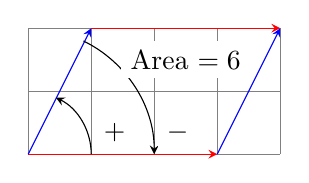
\begin{tikzpicture}[scale=.8]
\draw[help lines,step=1cm] (0,0) grid (4,2);
\draw[->,>=stealth,red] (0,0) -- (3,0);
\draw[->,>=stealth,red] [shift={(1,2)}](0,0) -- (3,0);
\draw[->,>=stealth,blue] (0,0) -- (1,2);
\draw[->,>=stealth,blue] [shift={(3,0)}](0,0) -- (1,2);
\draw[->,>=stealth] (0:1cm)  node[above right=1pt,fill=white]{\normalsize $+$} arc (0:64:1cm) ;
\draw[<-,>=stealth] (0:2cm)  node[above right=1pt,fill=white]{\normalsize $-$} arc (0:64:2cm) ;
\node[fill=white] at (2.5, 1.5) {Area $=6$}; 
\end{tikzpicture}

\vspace{2pt}
$\begin{vmatrix}{3}&{1}\\{0}&{2}\end{vmatrix}=6$ and $\begin{vmatrix}{1}&{3}\\{2}&0\end{vmatrix}=-6$
\end{center}
\caption{The determinant gives both area and direction. A counter clockwise rotation from column 1 to column 2 gives a positive determinant.\label{detfig}}
\end{figure}
%    }}

For a 3 by 3 matrix, the columns give the edges of a three dimensional parallelepiped and the determinant produces the volume of this object. The sign of the determinant is related to orientation. If you can use your right hand and place your index finger on the first vector, middle finger on the second vector, and thumb on the third vector, then the determinant is positive. 
For example, consider the matrix $A = \begin{bmatrix}\cl{1\\0\\0}&\cl{0\\2\\0}&\cl{0\\0\\3}\end{bmatrix}$.  Starting from the origin, each column represents an edge of the rectangular box 
$0\leq x\leq 1$, 
$0\leq y\leq 2$, 
$0\leq z\leq 3$ with volume (and determinant) $V=lwh=(1)(2)(3)=6$. The sign of the determinant is positive because if you place your index finger pointing in the direction (1,0,0) and your middle finger in the direction (0,2,0), then your thumb points upwards in the direction (0,0,3). 
If you interchange two of the columns, for example 
$B = \begin{bmatrix} \cl{0\\2\\0}&\cl{1\\0\\0}&\cl{0\\0\\3}\end{bmatrix}$, then the volume doesn't change since the shape is still the same. However, the sign of the determinant is negative because if you point your index finger in the direction (0,2,0) and your middle finger in the direction (1,0,0), then your thumb points down in the direction (0,0,-3). If you repeat this with your left hand instead of right hand, then your thumb points up.

\begin{problem}
\begin{enumerate}
\item Use determinants to find the area of the triangle with vertices $(0,0)$, $(-2,5)$, and $(3,4)$.
\item What would you change if you wanted to find the area of the triangle with vertices $(-3,1)$, $(-2,5)$, and $(3,4)$? Find this area.
\end{enumerate}
\end{problem}

\fi
%=========================================================
%End Matrix section that is printed if Valpo is on.
%=========================================================

\section{The Cross Product}
\large Topical Objective: \normalsize \\
\indent $\bullet$ perform the cross-product of vectors\\

\vskip0.2in

The dot product gave us a way of multiplying two vectors together, but the result was a number, not a vectors. We now define the cross product, which will allow us to multiply two vectors together to give us another vector.  We were able to define the dot product in all dimensions.  The cross product is only defined in $\mathbb{R}^3$. 

\begin{definition}[The Cross Product]
\marginpar{This definition is not really a definition.  It is actually a theorem.  If you use the formula given as the definition, then you would need to prove the three facts. We have the tools to give a complete proof of (1) and (3), but we would need a course in linear algebra to prove (2). It shouldn't be too much of a surprise that the cross product is related to area, since it is defined in terms of determinants}
The cross product of two vectors $\vec u = \left<u_1,u_2,u_3\right>$ and $\vec v = \left<v_1,v_2,v_3\right>$ is a new vector $\vec u\times \vec v$. This new vector is (1) orthogonal to both $\vec u$ and $\vec v$, (2) has a length equal to the area of the parallelogram whose sides are these two vectors, and (3) points in the direction your thumb points as you curl the base of your right hand from $\vec u$ to $\vec v$. The formula for the cross product is $$\vec u\times \vec v = \left<u_2v_3-u_3v_2,-(u_1v_3-u_3v_1),u_1v_2-u_2v_1\right> = \det\begin{bmatrix}\vec i & \vec j&\vec k\\ u_1&u_2&u_3\\ v_1&v_2&v_3\\\end{bmatrix}.$$
\end{definition}

\begin{problem} \instructor{Recommended as Pre-class} 
\marginpar{
	\thomasee{See 12.4: 1-8.} 
	\stewarts{See 12.4:1-7}
	}%
Let $\vec u=\langle 1,-2,3\rangle $ and $\vec v=\langle 2,0,-1\rangle$.  
\begin{enumerate}
\item Compute $\vec u\times \vec v$ and $\vec v\times \vec u$.  How are they related?
\item Compute $\vec u \cdot (\vec u\times \vec v)$ and $\vec v \cdot (\vec u\times \vec v)$. Why did you get the answer you got?
\item Compute $\vec u \times (2\vec u)$.  Why did you get the answer you got?
%\item Compute $|\vec u \times \vec v|$.  Compute the area of the parallelogram formed by $\vec u$ and $\vec v$ using trigonometry and $|\vec u|$, $|\vec v|$, and the angle $\theta$ between the two vectors. Compare your answer with $|\vec u \times \vec v|$.
\end{enumerate}
\end{problem}

\begin{problem} \instructor{Recommended as Pre-class}
\marginpar{
	\thomasee{See 12.4: 9-14.} 
	}%
Consider the vectors ${\ii}=(1,0,0)$, ${2\jj}=(0,2,0)$, and ${3\kk}=(0,0,3)$.
\begin{enumerate}
\item Compute $\ii\times {2\jj}$ and ${2\jj}\times {\ii}$.
\item Compute ${\ii}\times {3\kk}$ and ${3\kk}\times {\ii}$.
\item Compute ${2\jj}\times {3\kk}$ and ${3\kk}\times {2\jj}$.
\end{enumerate}
Give a geometric reason as to why some vectors above have a plus sign, and some have a minus sign.
\end{problem}

\begin{problem}  \instructor{Recommended as Pre-class}
\marginpar{
	\thomasee{See 12.4: 15-18.} 
	\stewarts{See 12.4: 29-32}
	}%
Let $P=(2,0,0)$, $Q=(0,3,0)$, and $R=(0,0,4)$. Find a vector that orthogonal to both $\vec {PQ}$ and $\vec {PR}$. Then find the area of the triangle $PQR$ [Hint: What shape does two triangles side-by-side make?]. Construct a 3D graph of this triangle. 
\end{problem}

\section{The Cross Product and Planes}
\large Topical Objectives \normalsize \\
\indent $\bullet$ use the normal vector to find the equation for a plane

\vskip0.2in

We will now combine the dot product with the cross product to develop an equation of a plane in 3D. 
Before doing so, let's look at what information we need to obtain a line in 2D, and a plane in 3D.  
To obtain a line in 2D, one way is to have 2 points. 
The next problem introduces the new idea by showing you how to find an equation of a line in 2D. 

\begin{problem}\label{prob:plane equation normal point}
Suppose the point $P=(1,2)$ lies on line $L$. Suppose that the angle between the line and the vector $\vec n=\left<3,4\right>$ is 90$^\circ$ (whenever this happens we say the vector $\vec n$ is normal to the line). Let $Q=(x,y)$ be another point on the line $L$. Use the fact that $\vec n$ is orthogonal to $\vec {PQ}$ to obtain an equation of the line $L$. 
\end{problem}

\note{Add a problem about the equation of a plane containing two vectors.}

\begin{problem}\label{plane equation three points}
\marginpar{
	\thomasee{See page 709.}
	\larsonfive{See Larson 11.5.} 
	\stewarts{See pages 819-822}
	}%
Let $P=(a,b,c)$ be a point on a plane in 3D. Let $\vec n=\langle A,B,C \rangle $ be a normal vector to the plane (so the angle between the plane and and $\vec n$ is 90$^\circ$).  Let $Q=(x,y,z)$ be another point on the plane.  Show that an equation of the plane through point $P$ with normal vector $\vec n$ is $$A(x-a)+B(y-b)+C(z-c)=0.$$
\end{problem}

%\newpage
%\noindent \Large After Class: \normalsize


\begin{problem}\label{plane equation 2 lines}
\marginpar{
	\larsonfive{See Larson 11.5:47--58 for more practice.}
	}%
Find an equation of the plane containing the lines $\vec r_1(t)=(1,3,0)t+(1,0,2)$ and $\vec r_2(t)=(2,0,-1)t+(2,3,2)$.
\end{problem}

\begin{problem}  
\marginpar{
	\thomasee{See 12.5: 21-28.}
	\larsonfive{See Larson 11.5:47--58 for more practice.} 
	\stewarts{See 12.5: 23-40}
	}%
Consider the three points $P=(1,0,0), Q=(2,0,-1), R=(0,1,3)$. Find an equation of the plane which passes through these three points.  [Hint: First find a normal vector to the plane.]
\end{problem}

\begin{problem}\label{prob:crossproduct normalvector}
 Consider the points $P=(2,-1,0)$, $Q=(0,2,3)$, and $R=(-1,2,-4)$.  
\begin{enumerate}
 \item Give an equation $(x,y,z)=(?,?,?)$ of the line through $P$ and $Q$.
 \item Give an equation of the line through $P$ and $R$.
 \item Give an equation of the plane through $P$, $Q$, and $R$. 
\end{enumerate}
\end{problem}

\begin{problem}  
\marginpar{
	\thomasee{See 12.5: 57-60.}
	\larsonfive{See Larson 11.5:91--92 for more practice.} 
	\stewarts{See 12.5: 23-40, 45-47}
	}%
Consider the two planes $x+2y+3z=4$ and $2x-y+z=0$.  These planes meet in a line.  Find a vector that is parallel to this line.  Then find a vector equation of the line.
\end{problem}


%\uday
\section{Projections and Their Applications}
\large Course Objective: \normalsize \\
\indent $\bullet$ See applications of multi-variable calculus

\vskip0.2in

Suppose a heavy box needs to be lowered down a ramp.  
The box exerts a downward force of 200 Newtons, which we will write in vector notation as $\vec F=\left<0,-200\right>$. 
The ramp was placed so that the box needs to be moved right 6 m, and down 3 m, so we need to get from the origin $(0,0)$ to the point $(6,-3)$.  This displacement can be written as $\vec d=\left<6,-3\right>$. The force $F$ acts straight down, which means the ramp takes some of the force. Our goal is to find out how much of the 200N the ramp takes, and how much force must be applied to prevent the box from sliding down the ramp (neglecting friction). We are going to break the force $\vec F$ into two components, one component in the direction of $\vec d$, and another component orthogonal to $\vec d$. 

\begin{problem}\label{prob:force intro}
Read the preceding paragraph.\\
We want to write $\vec F$ as the sum of two vectors: $\vec F = \vec w+\vec n$
\begin{itemize}
	\item where $\vec w$ is parallel to $\vec d$ 
	\item and $\vec n$ is orthogonal to $\vec d$
\end{itemize}
Since $\vec w$ is parallel to $\vec d$, we can write $\vec w=c\vec d$ for some unknown scalar $c$.\\
\begin{enumerate}
	\item Rewrite $\vec F$ in terms of $\vec d$
	\item Take the dot-product of both sides with $\vec d$
	\item Since $\vec n$ is orthogonal to $\vec d$ we know that $\vec n \cdot \vec d =$ ?
	\item Substitute and solve for the unknown $c$
\end{enumerate}
\end{problem}

The solution to the previous problem gives us the definition of a projection.

\begin{definition}
The projection of $\vec F$ onto $\vec d$, written $\proj_{\vec d}\vec F$, is defined as $$\proj_{\vec d}\vec F = \left(\frac{\vec F\cdot \vec d}{\vec d\cdot \vec d}\right)\vec d.$$
\end{definition}

\hrule

\begin{problem} 
\marginpar{
	\thomasee{See 12.3:1-8 (part d).} 
	\stewarts{See 12.3: 39-44}
	}%
Let $\vec u=(-1,2)$ and $\vec v=(3,4)$. Compute the $\proj_{\vec v}\vec u$. Draw $\vec u,$ $\vec v$, and $\proj_{\vec v}\vec u$ all on one set of axis. Then draw a line segment from the head of $\vec u$ to the head of the projection.\\

Now let $\vec w=(-2,0)$. Compute $\proj_{\vec v}\vec w$. Draw $\vec u,$ $\vec v$, and $\proj_{\vec v}\vec w$. Then draw a line segment from the head of $\vec w$ to the head of the projection.

\end{problem}

One application of projections pertains to the concept of work. Work is the transfer of energy. If a force $F$ acts through a displacement $d$, then the most basic definition of work is $W=Fd$, the product of the force and the displacement.  This basic definition has a few assumptions.
\begin{itemize}
\item The force $F$ must act in the same direction as the displacement.
\item The force $F$ must be constant throughout the entire displacement.
\item The displacement must be in a straight line.
\end{itemize}
Before the semester ends, we will be able to remove all 3 of these assumptions.  The next problem will show you how dot products help us remove the first assumption.

Recall the set up to problem \ref{prob:force intro}.  We want to lower a box down a ramp (which we will assume is frictionless). Gravity exerts a force of $\vec F=\left<0,-200\right>$ N. If we apply no other forces to this system, then gravity will do work on the box through a displacement of $\left<6,-3\right>$ m. The work done by gravity will transfer the potential energy of the box into kinetic energy (remember that work is a transfer of energy).  How much energy is transferred?

\begin{problem}[Projection Application: Work]\label{first work problem}
\marginpar{
	\thomasee{See 12.3: 24, 41-44.} 
	\stewarts{See 12.3:49-52}
	}% 
Find the amount of work done by the force $\vec F=\left<0,-200\right>$ through the displacement $\vec d=\left<6,-3\right>$. Find this by doing the following:
\begin{enumerate}
\item Find the projection of $\vec F$ onto $\vec d$. This tells you how much force acts in the direction of the displacement. Find the magnitude of this projection.
\item Since work equals $W=Fd$, multiply your answer above by $|\vec {d}|$.  
\item Now compute $\vec F\cdot \vec d$. You have just shown that $W=\vec F\cdot \vec d$ when $\vec F$ and $\vec d$ are not in the same direction.
\end{enumerate}
\end{problem}

%\newpage
%\noindent \Large After Class: \normalsize
%\section{More Planes}

\begin{problem}[Projection Application: Planes] 
\marginpar{
	\stewarts{See 12.5:69-72}
	}%
 Consider the points $P=(2,4,5)$, $Q=(1,5,7)$, and $R=(-1,6,8)$.
\begin{enumerate}
 \item What is the area of the triangle $PQR$. 
 \item Give a normal vector to the plane through these three points.
 \item What is the distance from the point $A=(1,2,3)$ to the plane $PQR$.  [Hint: Compute the projection of $\vec {PA}$ onto $\vec n$.  How long is it?] 
\end{enumerate}

 
\end{problem}



% \begin{problem}
%   Show that the distance from a point $Q$ to a plane (with normal vector {$\vec n$} and a point $P$) is given by $|\proj_{\vec n}\overrightarrow {PQ}|$. Draw a diagram illustrating your reasoning.
% \end{problem}

% \begin{problem}
%   Show that the distance from a line (with direction vector $\vec v_1$ passing through $P_1$) to a line (with direction vector $\vec v_2$ passing through $P_2$) is $|\proj_{\vec v_1\times\vec v_2}\overrightarrow {P_1P_2}|$. Draw a diagram illustrating your reasoning.
% \end{problem}

\note{Here are two more problems about dot and cross product, but they aren't central to the course.  Maybe these could be good problems for advanced students.  I saw these in Larson:

  \begin{problem} If the statement is true, explain why.  If it is false, give a counterexample.
    \begin{enumerate}
    \item If $\vec u \neq 0$ and $\vec u \times \vec v = \vec u \times \vec w$, then is $\vec v = \vec w$ always?
    \item If $\vec u \neq 0$, $\vec u\cdot \vec v = \vec u \cdot \vec w$,  and $\vec u \times \vec v = \vec u \times \vec w$, then is $\vec v = \vec w$ always?
    \end{enumerate}
  \end{problem}
}

\clearpage
